\section{Validation and controlled benchmarks}\label{sec:validation}

Before auditing published rough-volatility pricers, we validate every component of the framework against
closed-form analytic controls, independent high-precision quadrature, and known exact laws.

\paragraph{Analytic controls for Theorem~\ref{thm:tilted} (\textnormal{\lab{Arb-certified}})}
On the constant-kernel control ($k_u\equiv h$, $\norm{h}=1.2$, $\int a=0.235^2$), the 169-bit Arb
implementation of \eqref{eq:tilted_bracket} encloses the exact value
$100e^{-\norm{h}^2/8}\sqrt{\int a}\simeq19.628850$ volatility points with relative endpoint enclosure width of approximately
$3.38\times10^{-50}$. On the symmetric two-atom control $k_\pm=h\pm\varepsilon e$ ($e\perp h$,
$\norm{e}=1$, equal weights) for $\varepsilon\in\{0.1,0.2,0.4\}$, Arb reproduces the closed-form moment
ratio $m_2/m_1^2=\cosh(\varepsilon^2)$ and both endpoints to $3.5\times10^{-50}$, strictly contains the
independently integrated truth $e^{-\norm{h}^2/8}\sqrt{\int a}\,\E[\sqrt{e^{-\varepsilon^2/2}\cosh(\varepsilon Z)}]$,
and yields $(U-L)/(U\varepsilon^4)\in\{0.249993,0.249883,0.248149\}$, matching the sharp asymptotic
constant $\tfrac14$ of \eqref{eq:eps4_rate}.

\paragraph{Closed-form Pfaff ${}_2F_1$ evaluation and quadrature cross-check}
At $H=0.10$, $T=0.5$, $\Delta=30/365$, and $\eta_{\mathrm{P1}}=3.0$, the closed-form Arb inner products
\eqref{eq:nh2_pfaff}--\eqref{eq:hkx_pfaff} agree with independent adaptive numerical integration of
$C_0(x,y)$ (\texttt{scipy.integrate.quad}, tolerance $10^{-13}$) to relative differences
$7.75\times10^{-16}$ for $\ip{h_0}{\phi_{\Delta/3}}$ and $2.65\times10^{-16}$ for $\norm{h_0}^2$.
Two independent implementations of the Bourgey--De Marco--Gobet (2023) Theorem~2.2 futures expansion agree
to within $6.3\times10^{-5}$ volatility points across all eight headline parameter cells: our 169-bit Arb
kernel integration and a floating-point Gauss--Legendre routine matching the authors' public code
(Section~\ref{sec:vix_futures}). Run directly, the authors' published routine reproduces our Arb values to
within $5\times10^{-7}$ points once its quadrature is refined; at its default $30$-node setting it lies above
them by up to $\BDGDefaultExcessHi$ points, so the default would only enlarge the excesses reported below.

\paragraph{Mehler ledger and residual-to-output sandwich (\textnormal{\lab{exact-identity+quadrature}})}
On two-atom Wick-exponential configurations with known interaction $I=\pm1$, Theorem~\ref{thm:master}
is reproduced to $10^{-13}$; on five-atom signed fractional Brownian motion functionals ($H=0.3$,
$N\in\{2,3,4,\infty\}$), the ledger agrees with $2\times10^6$ Gaussian samples across Wick
exponential ($z=0.93$), exceedance ($z=1.56$), occupation ($z=-0.01$), and generic smooth ($z=1.00$)
non-linearities. Across all 24 test cases of Theorem~\ref{thm:sandwich} (Supplementary Figure~S1),
the ordering holds without exception: the lower bound captures $\SandLoSmooth$--$\SandHiSmooth\%$ of $P_\rho$ for smooth and
kinked outputs ($\SandLoOcc$--$\SandHiOcc\%$ for the occupation indicator), while the subspace Poincar\'e upper bound
overshoots by $\SandOverLo$--$\SandOverHi\%$ where finite.

\paragraph{Paired quantile-rate verification (\textnormal{\lab{statistical}$(0.95)$})}
To test Proposition~\ref{prop:condvar}(ii)--(iii) against an exact continuum truth, we evaluate the
$95\%$ quantile of $\Lambda=\int_0^1 B_H(s)^2\dd s$ (exact law by Karhunen--Lo\`eve and Imhof inversion,
variance verified to \EfiveTruthDisc) from $K=20{,}000$ exact samples of $n$-point midpoint observations
across $H\in\{0.1,0.3,0.5,0.75\}$ and $n\in\{4,16,64\}$ (full 12-cell breakdown in Supplementary Table~S2).
On identical draws, conditional Cantelli brackets with exact binomial order statistics are \EfivecBinALo--\EfivecBinAHi\
times narrower than the Riemann--$W_2$ baseline and \EfivecBinCLo--\EfivecBinCHi\ times narrower than
martingale-sharp endpoints, while maintaining empirical coverage at least \EfivecBinCov\ (nominal $0.95$).
Measuring the pure bias shift without sampling correction over $n=4,\dots,128$ ($K=200{,}000$,
Figure~\ref{fig:rates_cond}(b)) gives fitted exponents \EfivecSlopeCa\ (martingale budget) versus
\EfivecSlopeDa\ (conditional variance) at $H=0.1$, and \EfivecSlopeCb\ versus \EfivecSlopeDb\ at $H=0.3$,
directly confirming the $P^{1/2}$ versus $P^{1/3}$ ordering of Proposition~\ref{prop:condvar}(iii). Full
coverage, allocation, and supporting validation displays appear in the Supplementary Material.

\begin{figure}[!htbp]\centering
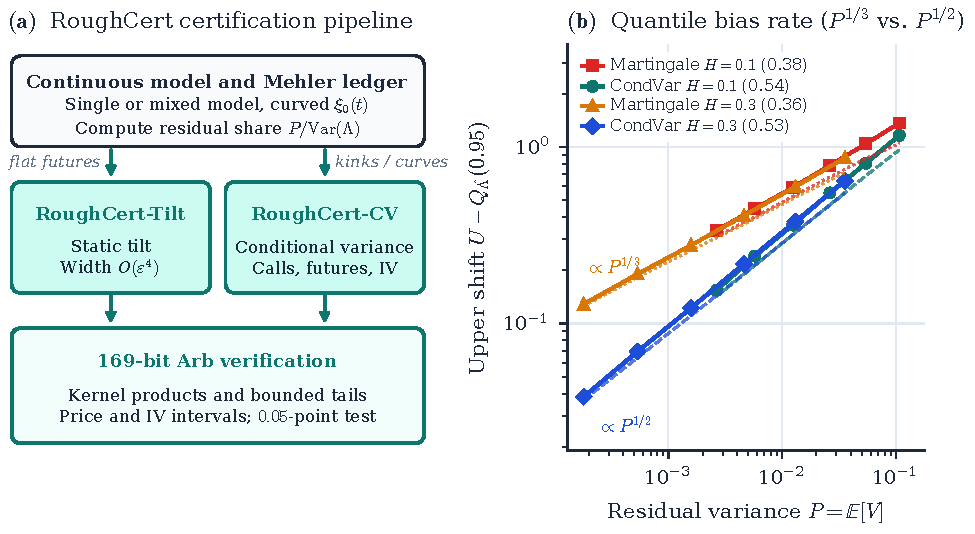
\includegraphics[width=\textwidth]{figures/fig_v3_01_pipeline_and_rates.pdf}
\caption{(a) Overview of the \RoughCert{} deterministic certification pipeline (\RoughCertTilt{} and
\RoughCertCV{}). (b) Upper quantile shift above $Q_{\hat\Lambda}(0.95)$ for $\int_0^1 B_H(s)^2\dd s$ versus
residual variance $P$ ($n=4,\dots,128$), confirming the $P^{1/3}$ versus $P^{1/2}$ local rates.}\label{fig:rates_cond}
\end{figure}
\ifTwoColumn\else\FloatBarrier\fi
